\section{Konzept 3}

\subsection{Idee}
\begin{figure}[h!]
	\centering
	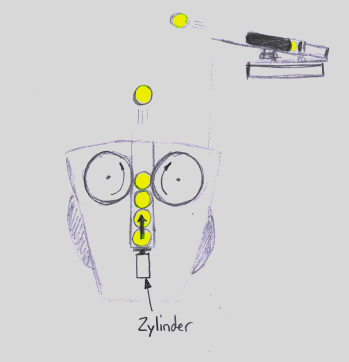
\includegraphics[width=0.4\textwidth]{../../fig/Wurfmaschine_Drehraeder.png}
	\caption{Aufbau mit zwei Rädern}
	\label{fig:drehradmaschine}
\end{figure}

Das dritte Konzept bedient sich einer unter Ballwurfmaschinen weit verbreiteten Methode Bälle zu beschleunigen. Zwei koaxial zueinander stehende Räder werden zum Drehen gebracht. Die Bälle müssen dann jeweils nur noch zwischen die Räder gebracht werden, um sich in Richtung der Drehrichtung zu beschleunigen.  

Als Variante dazu, würde sich ein Aufbau mit nur einem Drehrad anbieten.


\subsection{Annahmen}
TODO

\subsection{Risiken}
Variierende Klemmkraft: Die zu erwartenden Grössenunterschiede der Wurfgeschosse könnten, ohne geeignete Radbefestigung, zu unterschiedlichen Wurfweiten führen.
Unterschiedliche Drehzahlen: Dreht sich ein Rad schneller als das andere, könnte am Ball entstehender Drall die Wurfbahn beeinflussen.

\subsection{Bewertung}
Vorteile:
-Schnelligkeit
-Einstellbare Wurfweite

Nachteile: